\documentclass[border=10pt]{standalone}
\usepackage{tikz}
\usetikzlibrary{arrows.meta, calc}

\begin{document}
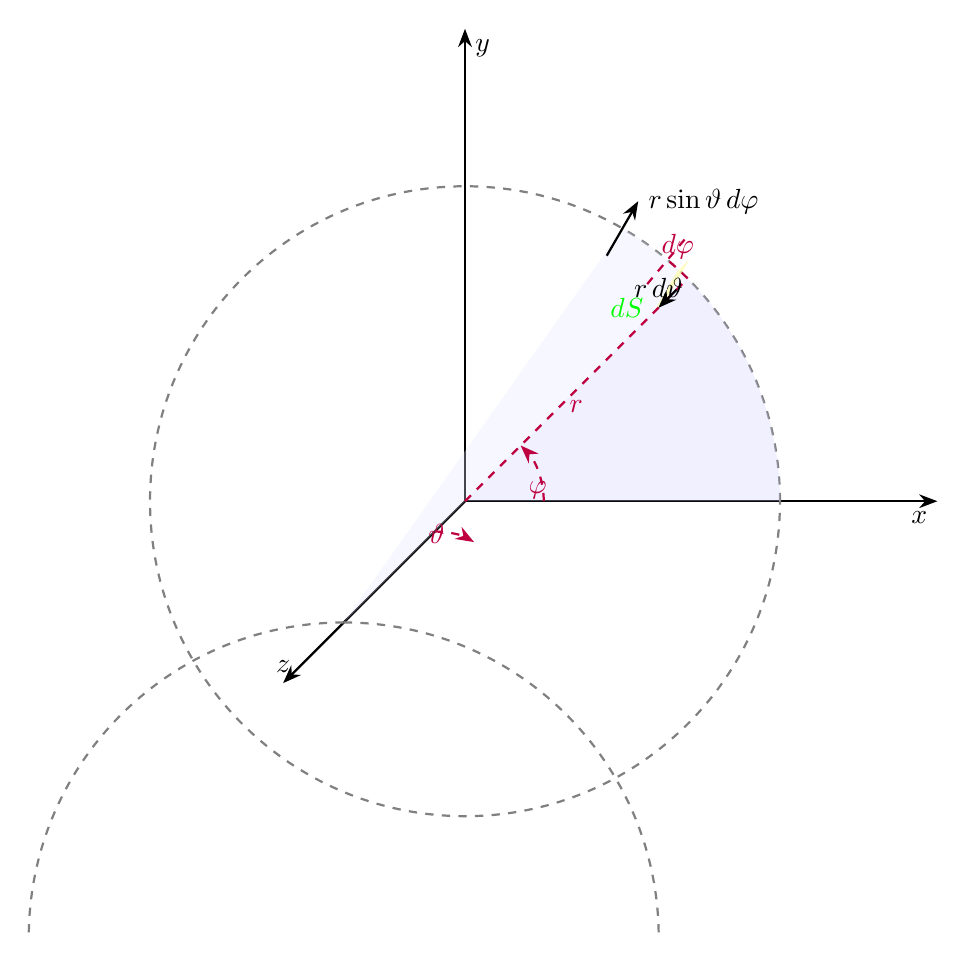
\begin{tikzpicture}[>=Stealth, thick, scale=2]

    % Coordinate axes
    \draw[->] (0,0,0) -- (3,0,0) node[anchor=north east] {$x$};
    \draw[->] (0,0,0) -- (0,3,0) node[anchor=north west] {$y$};
    \draw[->] (0,0,0) -- (0,0,3) node[anchor=south] {$z$};

    % Sphere outline (dashed)
    \draw[dashed, gray] (0,0,0) circle (2cm);
    \draw[dashed, gray] (0,0,2) arc (90:0:2cm);
    \draw[dashed, gray] (0,0,2) arc (90:180:2cm);

    % Spherical wedge (shaded)
    \fill[blue!20, opacity=0.3] 
        (0,0,0) -- 
        (2,0,0) arc (0:45:2cm) -- 
        (0,0,2) -- cycle;
    \fill[blue!10, opacity=0.3] 
        (0,0,0) -- 
        (45:2cm) arc (45:60:2cm) -- 
        (0,0,2) -- cycle;

    % Differential surface element
    \fill[yellow!40, opacity=0.6] 
        (45:1.8cm) -- 
        ++(0,0,0.2) -- 
        ++(60:0.3cm) -- 
        ++(0,0,-0.2) -- cycle;

    % Angle indicators
    \draw[dashed, purple] (0,0,0) -- (45:2cm) node[midway, below] {$r$};
    \draw[dashed, purple, ->] (0.5,0,0) arc (0:45:0.5cm) node[midway, below] {$\varphi$};
    \draw[dashed, purple, ->] (0,0,0.5) arc (90:60:0.5cm) node[midway, left] {$\vartheta$};

    % Differential element labels
    \draw[->, black] (45:1.9cm) -- ++(0,0,0.3) node[above] {$r\,d\vartheta$};
    \draw[->, black] (60:1.8cm) -- ++(60:0.4cm) node[right] {$r \sin\vartheta\,d\varphi$};
    \node at (50:1.6cm) [green] {$dS$};

    % Phi angle increment
    \draw[dashed, purple] (45:2cm) arc (45:50:2cm) node[midway, above] {$d\varphi$};
    \draw[dashed, purple] (50:1.8cm) -- (50:2.2cm);

\end{tikzpicture}
\end{document}